% Author: Izaak Neutelings (February 2020)
\documentclass[border=3pt,tikz]{standalone}
\usepackage{physics}
\usepackage{xcolor}
\usetikzlibrary{decorations.markings}
\tikzset{>=latex} % for LaTeX arrow head

\colorlet{Ecol}{orange!90!black}
\colorlet{Bcol}{violet!90}
\colorlet{Icol}{blue!70!black}
\colorlet{gausscol}{green!40!black}
\colorlet{gausscol2}{green!45!blue}
\tikzstyle{current}=[->,Icol,thick]
\colorlet{pluscol}{red!60!black}
\colorlet{minuscol}{blue!60!black}
\tikzstyle{anode}=[top color=red!20,bottom color=red!50,shading angle=20]
\tikzstyle{cathode}=[top color=blue!20,bottom color=blue!40,shading angle=20]
\tikzstyle{gauss surf}=[gausscol,top color=green!2,bottom color=green!80!black!70,shading angle=5,fill opacity=0.4]
\tikzstyle{metal}=[top color=black!15,bottom color=black!25,middle color=black!20,shading angle=10]
\tikzstyle{mydashes}=[dash pattern=on 1 off 1]
\tikzset{
  EFieldLine/.style={thick,Ecol,line cap=round,decoration={markings,
                     mark=at position #1 with {\arrow{latex}}},
                     postaction={decorate}},
  BFieldLine/.style={thick,Bcol,postaction={decorate},decoration={markings,
                     mark=at position #1 with {\arrow{latex}},
                     mark=at position #1+0.5 with {\arrow{latex}}}},
  EFieldLine/.default=0.5,
  BFieldLine/.default=0.4}
\usetikzlibrary{3d}

\begin{document}


% CAPACITOR 3D - displacement current derivation
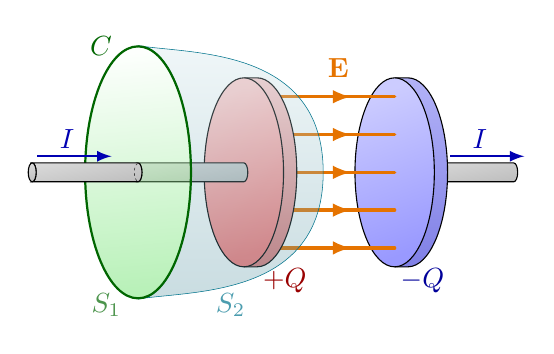
\begin{tikzpicture}[xscale=0.42]
  
  \def\RC{1.2}     % radius capacitor
  \def\RW{0.1*\RC} % radius wire
  \def\RA{1.6}     % radius ampere loop
  \def\D{2.6*\RA}  % distance between plates
  \def\T{0.4}      % plate thickness
  \def\L{2*\RA}    % wire length
  \def\NE{5}       % number of electric field lines
  
  % CATHODE WIRE
  \draw[metal]
    (\D+\T,\RW) --++ (\L,0) arc (90:-90:\RW) --++ (-\L,0);
  
  % CATHODE
  \draw[cathode,top color=blue!90!black!30,bottom color=blue!80!black!50]
    (\D,\RC) --++ (\T,0) arc (90:-90:\RC) --++ (-\T,0);
  \draw[cathode] (\D,0) circle (\RC);
  
  % ELECTRIC FIELD
  \foreach \i [evaluate={\y=-\RC+(\i-0.5)*(2*\RC)/\NE);}] in {1,...,\NE}{
    \draw[EFieldLine={0.68},very thick] (0,\y) --++ (\D,0);
  }
  \node[Ecol,above] at (0.59*\D,0.9*\RC) {$\vb{E}$};
  
  % ANODE
  \draw[anode,top color=red!90!black!20,bottom color=red!80!black!50]
    (-\T,\RC) --++ (\T,0) arc (90:-90:\RC) --++ (-\T,0);
  \draw[anode] (-\T,0) circle (\RC);
  
  % ANODE WIRE LEFT
  \draw[metal]
    (-\T,\RW) arc (90:-90:\RW) --++ (-\L,0) arc (-90:90:\RW) -- cycle;
  
  % SURFACE
  \draw[gauss surf,very thin,fill opacity=0.3,gausscol2,
        top color=gausscol2!20,bottom color=gausscol2!80!black!70]
    %(-\T-\L,\RA) arc (90:-90:{1.2*(\T+\L+\RA)} and {\RA}) arc (-90:90:\RA);
    (-\T-\L,1.006*\RA) to[out=-4,in=90,looseness=0.7] (\T+\RA,0) to[out=-90,in=4,looseness=0.7] (-\T-\L,-1.006*\RA) arc (-90:90:1.006*\RA);
  \draw[gauss surf,thick]
    (-\T-\L,0) circle (\RA);
  \node[gausscol] at (-\T-\L-0.7*\RA,\RA) {$C$};
  \node[gausscol!70] at (-\T-\L-0.6*\RA,-1.05*\RA) {$S_1$};
  \node[gausscol2!70] at (-0.5*\RA,-1.05*\RA) {$S_2$};
  \node[pluscol] at (0.7*\RC,-1.15*\RC) {$+Q$};
  \node[minuscol] at (\D+0.7*\RC,-1.15*\RC) {$-Q$};
  
  % ANODE WIRE RIGHT
  \draw[metal]
    (-\T-\L,\RW) arc (90:-90:\RW) --++ (-\L,0) arc (-90:90:\RW) -- cycle;
  \draw[mydashes,black!80,very thin]
    (-\T-\L,0.94*\RW) arc (90:270:0.94*\RW);
  \draw[metal]
    (-\T-2*\L,0) circle (\RW);
  
  % CURRENT
  \draw[current] (-\T-1.95*\L,1.7*\RW) --++ (0.7*\L,0) node[pos=0.4,above=-1] {$I$};
  \draw[current] (\D+\RC+0.15*\L,1.7*\RW) --++ (0.7*\L,0) node[pos=0.4,above=-1] {$I$};
  
\end{tikzpicture}


% CAPACITOR 3D - displacement current derivation (cylinder)
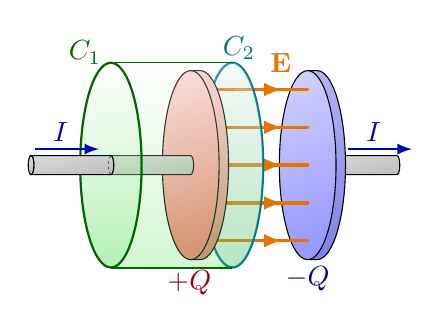
\begin{tikzpicture}[xscale=0.3]
  
  \def\RC{1.2}     % radius capacitor
  \def\RW{0.1*\RC} % radius wire
  \def\RA{1.3}     % radius ampere loop
  \def\D{3.5*\RA}  % distance between plates
  \def\T{0.4}      % plate thickness
  \def\L{2.6*\RA}  % wire length
  \def\NE{5}       % number of electric field lines
  \def\Sx{0.3*\D}  % x position S2
  
  % CATHODE WIRE
  \draw[metal]
    (\D+\T,\RW) --++ (\L,0) arc (90:-90:\RW) --++ (-\L,0);
  
  % CATHODE
  \draw[cathode,top color=blue!90!black!30,bottom color=blue!80!black!50]
    (\D,\RC) --++ (\T,0) arc (90:-90:\RC) --++ (-\T,0);
  \draw[cathode] (\D,0) circle (\RC);
  
  % ELECTRIC FIELD
  \foreach \i [evaluate={\y=-\RC+(\i-0.5)*(2*\RC)/\NE);}] in {1,...,\NE}{
    \draw[EFieldLine={0.76},very thick] (0,\y) --++ (\D,0);
  }
  \node[Ecol,above] at (0.75*\D,0.88*\RC) {$\vb{E}$};
  
  % SURFACE S2
  \draw[gauss surf,thick,fill opacity=0.2,gausscol2,
        top color=gausscol2!20,bottom color=gausscol2!80!black!70]
    (\Sx,0) circle (\RA);
  \foreach \i [evaluate={\y=-\RC+(\i-0.5)*(2*\RC)/\NE);}] in {1,...,\NE}{
    \draw[Ecol,very thick,line cap=round] (0,\y) --++ (\Sx,0);
  }
  
  % ANODE
  \draw[anode,top color=red!90!black!20,bottom color=red!80!black!50]
    (-\T,\RC) --++ (\T,0) arc (90:-90:\RC) --++ (-\T,0);
  \draw[anode] (-\T,0) circle (\RC);
  
  % ANODE WIRE LEFT
  \draw[metal]
    (-\T,\RW) arc (90:-90:\RW) --++ (-\L,0) arc (-90:90:\RW) -- cycle;
  
  % SURFACE S1
  \draw[gauss surf,draw=none,fill opacity=0.25]
     (\Sx-0.01,\RA) arc(90:-90:\RA) -- (-\T-\L,-\RA) arc(-90:90:\RA);
  \draw[gausscol,thin]
    (\Sx,\RA+0.007) -- (-\T-\L,\RA+0.007)
    (\Sx,-\RA-0.007) -- (-\T-\L,-\RA-0.007);
  \draw[gauss surf,thick]
    (-\T-\L,0) circle (\RA);
  \node[gausscol,left=0] at (-\T-\L,1.10*\RA) {$C_1$};
  \node[gausscol2,right=-7] at (\Sx,1.14*\RA) {$C_2$};
  %\node[gausscol!70] at (-\T-\L-0.6*\RA,-1.05*\RA) {$S_1$};
  %\node[gausscol2!70] at (\Sx+0.2*\D,-1.05*\RA) {$S_2$};
  \node[pluscol] at (-0.1*\D,-1.25*\RC) {$+Q$};
  \node[minuscol] at (1.0*\D,-1.20*\RC) {$-Q$};
  
  % ANODE WIRE RIGHT
  \draw[metal]
    (-\T-\L,\RW) arc (90:-90:\RW) --++ (-\L,0) arc (-90:90:\RW) -- cycle;
  \draw[mydashes,black!80,very thin]
    (-\T-\L,0.94*\RW) arc (90:270:0.94*\RW);
  \draw[metal]
    (-\T-2*\L,0) circle (\RW);
  
  % CURRENT
  \draw[current] (-\T-1.95*\L,1.7*\RW) --++ (0.8*\L,0) node[pos=0.4,above=-1] {$I$};
  \draw[current] (\D+\RC+0.15*\L,1.7*\RW) --++ (0.8*\L,0) node[pos=0.4,above=-1] {$I$};
  
\end{tikzpicture}


% CAPACITOR 3D - magnetic fields
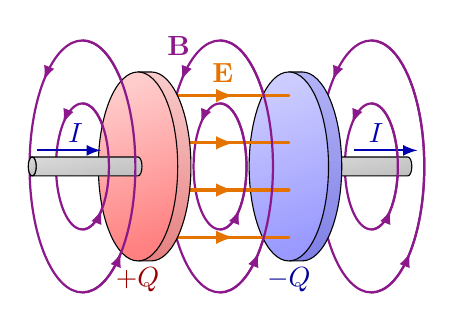
\begin{tikzpicture}[xscale=0.42]
  
  \def\RC{1.2}     % radius capacitor
  \def\RW{0.1*\RC} % radius wire
  \def\RA{1.6}     % radius ampere loop
  \def\D{2.6*\RA}  % distance between plates
  \def\T{0.4}      % plate thickness
  \def\L{2*\RA}    % wire length
  \def\NE{4}       % number of electric field lines
  \def\NB{2}       % number of magnetic field lines
  
  % MAGNETIC FIELD LINES back
  \foreach \x in {-0.5*\D,0.5*\D,1.6*\D}{
    \foreach \i [evaluate={\r=\i*\RA/\NB);}] in {1,...,\NB}{
      \draw[BFieldLine={0.35}] (\x,0) circle (\r);
    }
  }
  
  % CATHODE WIRE
  \draw[metal]
    (\D+\T,\RW) --++ (\L,0) arc (90:-90:\RW) --++ (-\L,0);
  
  % CATHODE
  \draw[cathode,top color=blue!90!black!30,bottom color=blue!80!black!50]
    (\D,\RC) --++ (\T,0) arc (90:-90:\RC) --++ (-\T,0);
  \draw[cathode] (\D,0) circle (\RC);
  
  % ELECTRIC FIELD
  \foreach \i [evaluate={\y=-\RC+(\i-0.5)*(2*\RC)/\NE);}] in {1,...,\NE}{
    \draw[EFieldLine={0.6},very thick] (0,\y) --++ (\D,0);
  }
  \node[Ecol,above] at (0.52*\D,0.78*\RC) {$\vb{E}$};
  \node[Bcol,above] at (0.20*\D,0.80*\RA) {$\vb{B}$};
  
  % ANODE
  \draw[anode,top color=red!90!black!20,bottom color=red!80!black!50]
    (-\T,\RC) --++ (\T,0) arc(90:-90:\RC) --++ (-\T,0);
  \draw[anode] (-\T,0) circle (\RC);
  
  % ANODE WIRE LEFT
  \draw[metal]
    (-\T,\RW) arc (90:-90:\RW) --++ (-\L,0) arc (-90:90:\RW) -- cycle;
  \draw[metal]
    (-\T-\L,0) circle (\RW);
  
  % SURFACE
  \node[pluscol] at (-0.1*\D,-1.2*\RC) {$+Q$};
  \node[minuscol] at (1.0*\D,-1.2*\RC) {$-Q$};
  
  % CURRENT
  \draw[current]
    (-\T-0.95*\L,1.7*\RW) --++ (0.6*\L,0) node[pos=0.6,above=-1] {$I$};
  \draw[current]
    (\D+\RC+0.24*\L,1.7*\RW) --++ (0.6*\L,0) node[pos=0.35,above=-1] {$I$};
  
  % MAGNETIC FIELD LINES front
  \foreach \x in {-0.5*\D,0.5*\D,1.6*\D}{
    \foreach \i [evaluate={\r=\i*\RA/\NB);}] in {1,...,\NB}{
      \draw[Bcol,thick] (\x,\r) arc(90:-90:\r);
    }
  }
  
\end{tikzpicture}


\end{document}